%%%%%%%%%%%%%%%%%%%%%%%%%%%%%%%%%%%%%%%%%
% Beamer Presentation
% LaTeX Template
% Version 1.0 (10/11/12)
%
% This template has been downloaded from:
% http://www.LaTeXTemplates.com
%
% License:
% CC BY-NC-SA 3.0 (http://creativecommons.org/licenses/by-nc-sa/3.0/)
%
%%%%%%%%%%%%%%%%%%%%%%%%%%%%%%%%%%%%%%%%%

%----------------------------------------------------------------------------------------
%	PACKAGES AND THEMES
%----------------------------------------------------------------------------------------

\documentclass[UTF8,aspectratio=169,14pt]{ctexbeamer}

\usepackage{hyperref}
\hypersetup{
	colorlinks=true,
	linkcolor=red,
	anchorcolor=blue,
	citecolor=green
}

\mode<presentation> {
	
	% The Beamer class comes with a number of default slide themes
	% which change the colors and layouts of slides. Below this is a list
	% of all the themes, uncomment each in turn to see what they look like.
	
	%\usetheme{default}
	%\usetheme{AnnArbor}
	%\usetheme{Antibes}
	%\usetheme{Bergen}
	%\usetheme{Berkeley}
	%\usetheme{Berlin}
	%\usetheme{Boadilla}
	%\usetheme{CambridgeUS}
	%\usetheme{Copenhagen}
	%\usetheme{Darmstadt}
	%\usetheme{Dresden}
	%\usetheme{Frankfurt}
	%\usetheme{Goettingen}
	%\usetheme{Hannover}
	%\usetheme{Ilmenau}
	%\usetheme{JuanLesPins}
	%\usetheme{Luebeck}
	\usetheme{Madrid}
	%\usetheme{Malmoe}
	%\usetheme{Marburg}
	%\usetheme{Montpellier}
	%\usetheme{PaloAlto}
	%\usetheme{Pittsburgh}
	%\usetheme{Rochester}
	%\usetheme{Singapore}
	%\usetheme{Szeged}
	%\usetheme{Warsaw}
	
	% As well as themes, the Beamer class has a number of color themes
	% for any slide theme. Uncomment each of these in turn to see how it
	% changes the colors of your current slide theme.
	
	%\usecolortheme{albatross}
	%\usecolortheme{beaver}
	%\usecolortheme{beetle}
	%\usecolortheme{crane}
	%\usecolortheme{dolphin}
	%\usecolortheme{dove}
	%\usecolortheme{fly}
	%\usecolortheme{lily}
	%\usecolortheme{orchid}
	%\usecolortheme{rose}
	%\usecolortheme{seagull}
	%\usecolortheme{seahorse}
	%\usecolortheme{whale}
	%\usecolortheme{wolverine}
	
	%\setbeamertemplate{footline} % To remove the footer line in all slides uncomment this line
	%\setbeamertemplate{footline}[page number] % To replace the footer line in all slides with a simple slide count uncomment this line
	
	%\setbeamertemplate{navigation symbols}{} % To remove the navigation symbols from the bottom of all slides uncomment this line
}

\usepackage{graphicx} % Allows including images
\graphicspath{{./figs/}}
\usepackage{booktabs} % Allows the use of \toprule, \midrule and \bottomrule in tables
\usepackage{longtable}
\usepackage{listings}
\usepackage{xcolor}
\lstset{numbers=left, %设置行号位置
	numberstyle=\tiny, %设置行号大小
	keywordstyle=\color{blue}, %设置关键字颜色
	commentstyle=\color[cmyk]{1,0,1,0}, %设置注释颜色
	frame=single, %设置边框格式
	escapeinside=``, %逃逸字符(1左面的键),用于显示中文
	%breaklines, %自动折行
	extendedchars=false, %解决代码跨页时,章节标题,页眉等汉字不显示的问题
	xleftmargin=2em,xrightmargin=2em, aboveskip=1em, %设置边距
	tabsize=4, %设置tab空格数
	showspaces=false %不显示空格
}
% Fonts
% \usepackage{libertine}
% \setmonofont{Courier}
\setCJKsansfont[ItalicFont=Noto Serif CJK SC Black, BoldFont=Noto Sans CJK SC Black]{Noto Sans CJK SC}


%----------------------------------------------------------------------------------------
% TITLE PAGE
%----------------------------------------------------------------------------------------

\title[第22讲]{第二十二讲 :异步编程(Asynchronous Programming)}  % The short title appears at the bottom of every slide, the full title is only on the title page
\subtitle{第5节:Waker and Reactor}
\author{向勇、陈渝、李国良} % Your name
\institute[清华大学] % Your institution as it will appear on the bottom of every slide, may be shorthand to save space
{
  清华大学计算机系 \\ % Your institution for the title page
  \medskip
  \textit{xyong,yuchen,liguoliang@tsinghua.edu.cn} % Your email address
}
\date{\today} % Date, can be changed to a custom date

\begin{document}

\begin{frame}
\titlepage % Print the title page as the first slide
\end{frame}

%----------------------------------------------
% \begin{frame}
% \frametitle{提纲} % Table of contents slide, comment this block out to remove it
% \tableofcontents % Throughout your presentation, if you choose to use \section{} and \subsection{} commands, these will automatically be printed on this slide as an overview of your presentation

%% itemize
% Ref:
%     \begin{itemize}
%         \item \href{}{xxxx}
%     \end{itemize}
% \end{frame}
%----------------------------------------------
%%  PRESENTATION SLIDES
%----------------------------------------------
\section{第5节:Waker and Reactor} % Sections can be created in order to organize your presentation into discrete blocks, all sections and subsections are automatically printed in the table of contents as an overview of the talk
%----------------------------------------------
%\subsection{xxxx} % A subsection can be created just before a set of slides with a common theme to further break down your presentation into chunks
%----------------------------------------------
\begin{frame}[fragile]
    \frametitle{Waker}
%    \framesubtitle{xxxx}
% ### 21.5 Waker and Reactor
% 
% Ref: https://cfsamson.github.io/books-futures-explained/2_waker_context.html#waker-and-context
% 
% #### Waker
% 
% Ref: https://cfsamson.github.io/books-futures-explained/2_waker_context.html#the-waker
% 
%% itemize
    \begin{itemize}
        \item The $Waker$ type allows for a loose coupling between the reactor-part and the executor-part of a runtime \pause
        \item By having a wake up mechanism that is {\color{red}not} tied to the thing that executes the future, runtime-implementors can come up with interesting new wake-up mechanisms \pause
        \item Creating a `Waker` involves creating a `vtable` which allows us to use dynamic dispatch to call methods on a {\color{red}type erased} trait object we construct our selves
    \end{itemize}

\end{frame}
%----------------------------------------------
\begin{frame}[fragile]
    \frametitle{Fat pointers in Rust}
%    \framesubtitle{xxxx}
% #### Fat pointers in Rust
% 
% Ref: https://cfsamson.github.io/books-futures-explained/2_waker_context.html#fat-pointers-in-rust
% 
{\color{red}Example `\&[i32]`}
 
 %% itemize
     \begin{itemize}
         \item The first 8 bytes is the actual pointer to the first element in the array (or part of an array the slice refers to)
         \item The second 8 bytes is the length of the slice.
     \end{itemize} \pause
 
{\color{red}Example `\&dyn SomeTrait`}
 
 %% itemize
     \begin{itemize}
         \item The first 8 bytes points to the `data` for the trait object
         \item The second 8 bytes points to the `vtable` for the trait object
     \end{itemize} \pause
 
{\color{red}Trait object}

%% itemize
    \begin{itemize}
        \item `\&dyn SomeTrait` is a reference to a trait, or what Rust calls a {\color{red}trait object}.
        \item Implement `Waker:` we'll actually set up a `vtable`
    \end{itemize} \pause

Example:

%% itemize
    \begin{itemize}
        \item \href{https://cfsamson.github.io/books-futures-explained/2_waker_context.html}{Fat pointers in Rust}
    \end{itemize}

\end{frame}
%----------------------------------------------
\begin{frame}[fragile]
    \frametitle{Reactor}
%    \framesubtitle{xxxx}
% #### Reactor
% 
% Ref: https://cfsamson.github.io/books-futures-explained/6_future_example.html#the-reactor
% https://docs.rs/tokio/0.1.22/tokio/reactor/index.html
% 
%% itemize
    \begin{itemize}
        \item To actually abstract over this interaction with the outside world in an asynchronous way \pause
    	\begin{itemize}
    	    \item Receive events from the operating system or peripherals
    	    \item Forward them to waiting tasks
    	\end{itemize} \pause

        \item \href{https://github.com/tokio-rs/mio}{Mio}: Library of reactors in Rust \pause
    	\begin{itemize}
    	    \item Provide non blocking APIs and event notification for several platforms
    	\end{itemize}
    \end{itemize}

\end{frame}
%----------------------------------------------
\begin{frame}[fragile]
    \frametitle{Reactor example}
%    \framesubtitle{xxxx}
% #### Reactor example
% 
    \begin{itemize}
        \item The example task is a {\color{red}timer} that only {\color{red}spawns a thread} and puts it to sleep for the number of seconds we specify. \pause
        \item The reactor we create here will create a {\color{red}leaf-future} representing each timer. \pause
        \item In return the Reactor receives a {\color{red}waker} which it will call once the task is finished. \pause
    \end{itemize}
% 
%% itemize
    \begin{itemize}
        \item \href{https://cfsamson.github.io/books-futures-explained/6_future_example.html}{Our Reactor}
    	\begin{itemize}
    	    \item Be dependent on thread::spawn
    	\end{itemize}
    \end{itemize}

\end{frame}
%----------------------------------------------
\begin{frame}[fragile]
    \frametitle{Async implementation in kernel mode}
%    \framesubtitle{xxxx}
% #### Async implementation in kernel mode
% 
% Ref: https://os.phil-opp.com/async-await/#simple-executor
% 
\begin{block}{}
    \begin{verbatim}
// in src/task/simple_executor.rs
pub struct SimpleExecutor {
    task_queue: VecDeque<Task>,
}
impl SimpleExecutor {
    pub fn new() -> SimpleExecutor {
        SimpleExecutor {
            task_queue: VecDeque::new(),
        }
    }
    pub fn spawn(&mut self, task: Task) {
        self.task_queue.push_back(task)
    }
}
    \end{verbatim}
\end{block}
% 
%% itemize
    \begin{itemize}
        \item Only dependent on queue, No dependent on thread
    \end{itemize}

\end{frame}
%----------------------------------------------
\begin{frame}[fragile]
    \frametitle{Asynchronous task based on the keyboard interrupt}
%    \framesubtitle{xxxx}
% #### Asynchronous task based on the keyboard interrupt
% 
% Ref: https://os.phil-opp.com/async-await/#async-keyboard-input
% 
%% itemize
    \begin{itemize}
        \item The executor has proper support for `Waker` notifications
    	\begin{itemize}
    	    \item The simple executor does not utilize the `Waker` notifications
    	    \item Simply loops over all tasks until they are done
    	\end{itemize} \pause

        \item Create an asynchronous task based on the keyboard interrupt
%    \end{itemize}
% 
%% figure
    \begin{figure}
    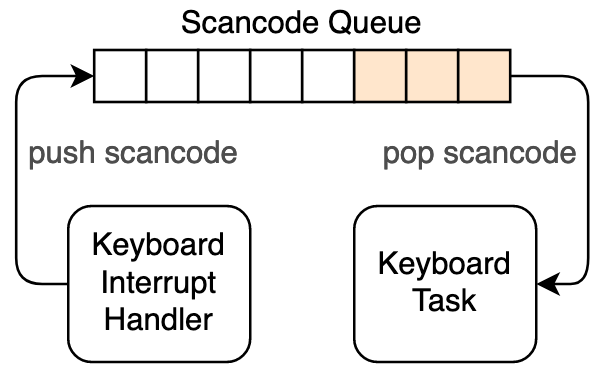
\includegraphics[width=0.35\linewidth]{figs/scancode-queue.png}
%    \caption{xxxx}
    \end{figure} \pause
% ![scancode-queue](figs/scancode-queue.svg)

%    \begin{itemize}
        \item A simple implementation of that queue could be a mutex-protected \href{https://doc.rust-lang.org/stable/alloc/collections/vec_deque/struct.VecDeque.html}{`VecDeque`}
    	\begin{itemize}
    	    \item Using mutexes in interrupt handlers is not a good idea since it can easily lead to deadlocks.
    	\end{itemize} \pause

        \item Example: \href{https://github.com/phil-opp/blog_os/blob/post-12/src/task/keyboard.rs}{Keyboard future}
    \end{itemize}

\end{frame}
%----------------------------------------------
\begin{frame}[fragile]
    \frametitle{Complete Example}
%    \framesubtitle{xxxx}
% #### Complete Example
% 
% Ref: https://cfsamson.github.io/books-futures-explained/8_finished_example.html#our-finished-code
% 
%% itemize
    \begin{itemize}
        \item \href{https://cfsamson.github.io/books-futures-explained/8_finished_example.html}{Finished Example}
    \end{itemize}
\end{frame}
%----------------------------------------------
\end{document}
